\documentclass{article}
% packages
\usepackage{amsmath,amssymb}
\usepackage{graphicx}
\usepackage{hyperref}

% directory of figures
%\graphicspath{ {figs} }

% latin bold lower
\newcommand{\ba}{\mathbf{a}} 
\newcommand{\bc}{\mathbf{c}} 
\newcommand{\be}{\mathbf{e}} 
\newcommand{\bh}{\mathbf{h}} 
\newcommand{\bp}{\mathbf{p}} 
\newcommand{\bt}{\mathbf{t}} 
\newcommand{\bs}{\mathbf{s}} 
\newcommand{\bu}{\mathbf{u}} 
\newcommand{\bv}{\mathbf{v}} 
\newcommand{\bw}{\mathbf{w}} 
\newcommand{\bx}{\mathbf{x}} 
\newcommand{\by}{\mathbf{y}} 
\newcommand{\bz}{\mathbf{z}} 
\newcommand{\bm}{\mathbf{m}} 

% latin bold upper
\newcommand{\bA}{\mathbf{A}} 
\newcommand{\bB}{\mathbf{B}} 
\newcommand{\bC}{\mathbf{C}} 
\newcommand{\bI}{\mathbf{I}} 
\newcommand{\bJ}{\mathbf{J}} 
\newcommand{\bL}{\mathbf{L}} 
\newcommand{\bM}{\mathbf{M}} 
\newcommand{\bP}{\mathbf{P}}
\newcommand{\bQ}{\mathbf{Q}} 
\newcommand{\bR}{\mathbf{R}} 
\newcommand{\bT}{\mathbf{T}} 
\newcommand{\bU}{\mathbf{U}} 
\newcommand{\bV}{\mathbf{V}} 
\newcommand{\bW}{\mathbf{W}} 
\newcommand{\bX}{\mathbf{X}} 
\newcommand{\bY}{\mathbf{Y}} 
\newcommand{\bZ}{\mathbf{Z}} 

% latin cal upper
\newcommand{\cF}{\mathcal{F}} 
\newcommand{\cG}{\mathcal{G}} 
\newcommand{\cI}{\mathcal{I}} 
\newcommand{\cL}{\mathcal{L}} 
\newcommand{\cM}{\mathcal{M}} 
\newcommand{\cN}{\mathcal{N}} 
\newcommand{\cS}{\mathcal{S}} 
\newcommand{\cT}{\mathcal{T}} 
\newcommand{\cW}{\mathcal{W}} 
\newcommand{\cX}{\mathcal{X}} 
\newcommand{\cZ}{\mathcal{Z}} 

% latin bb upper
\newcommand{\bbE}{\mathbb{E}} 
\newcommand{\bbI}{\mathbb{I}} 
\newcommand{\bbP}{\mathbb{P}} 
\newcommand{\bbR}{\mathbb{R}}
\newcommand{\bbX}{\mathbb{X}} 
\newcommand{\bbY}{\mathbb{Y}}
\newcommand{\bbW}{\mathbb{W}} 

% greek bold lower
\newcommand{\bepsilon}{\boldsymbol{\epsilon}} 
\newcommand{\btheta}{\boldsymbol{\theta}} 
\newcommand{\blambda}{\boldsymbol{\lambda}} 
\newcommand{\bpi}{\boldsymbol{\pi}} 
\newcommand{\bmu}{\boldsymbol{\mu}} 
\newcommand{\bsigma}{\boldsymbol{\sigma}} 
\newcommand{\bphi}{\boldsymbol{\phi}} 

% greek bold upper
\newcommand{\bSigma}{\boldsymbol{\Sigma}} 

\DeclareMathOperator*{\argmin}{arg\,min}
\DeclareMathOperator*{\argmax}{arg\,max}

% transpose
\newcommand{\T}{^{\text{\tiny\sffamily\upshape\mdseries T}}}

% if you need to pass options to natbib, use, e.g.:
\PassOptionsToPackage{numbers, sort, compress}{natbib}
% before loading neurips_2024


% ready for submission
%\usepackage{neurips_2024}


% to compile a preprint version, e.g., for submission to arXiv, add add the
% [preprint] option:
\usepackage[preprint]{neurips_2024}


% to compile a camera-ready version, add the [final] option, e.g.:
%     \usepackage[final]{neurips_2024}


% to avoid loading the natbib package, add option nonatbib:
%    \usepackage[nonatbib]{neurips_2024}


\usepackage[utf8]{inputenc} % allow utf-8 input
\usepackage[T1]{fontenc}    % use 8-bit T1 fonts
\usepackage{hyperref}       % hyperlinks
\usepackage{url}            % simple URL typesetting
\usepackage{booktabs}       % professional-quality tables
\usepackage{amsfonts}       % blackboard math symbols
\usepackage{nicefrac}       % compact symbols for 1/2, etc.
\usepackage{microtype}      % microtypography
\usepackage{xcolor}         % colors

%%%

\usepackage{subcaption}
\usepackage{graphicx}
\usepackage{multirow}
\usepackage{amsmath,amssymb,amsfonts}
\usepackage{amsthm}
\usepackage{mathrsfs}
\usepackage{xcolor}
\usepackage{textcomp}
\usepackage{manyfoot}
\usepackage{booktabs}
\usepackage{algorithm}
\usepackage{algorithmicx}
\usepackage{algpseudocode}
\usepackage{listings}
\usepackage{caption}
\usepackage{wrapfig}
\usepackage{picinpar}

\captionsetup[figure]{width=0.8\textwidth}

\newtheorem{theorem}{Theorem} % continuous numbers
%%\newtheorem{theorem}{Theorem}[section] % sectionwise numbers
%% optional argument [theorem] produces theorem numbering sequence instead of independent numbers for Proposition
\newtheorem{proposition}[theorem]{Proposition}% 
\newtheorem{lemma}{Lemma}% 
%%\newtheorem{proposition}{Proposition} % to get separate numbers for theorem and proposition etc.

\newtheorem{example}{Example}
\newtheorem{remark}{Remark}

\newtheorem{definition}{Definition}
\newtheorem{assumption}{Assumption}

%%%

\title{Detecting Manual Alterations in Biological Image Data 
Using Contrastive Learning and Pairwise Image Comparison}


% The \author macro works with any number of authors. There are two commands
% used to separate the names and addresses of multiple authors: \And and \AND.
%
% Using \And between authors leaves it to LaTeX to determine where to break the
% lines. Using \AND forces a line break at that point. So, if LaTeX puts 3 of 4
% authors names on the first line, and the last on the second line, try using
% \AND instead of \And before the third author name.


\author{%
  Georgii Nekhoroshkov\\
  MIPT\\
  Moscow, Russia\\
  \texttt{nekhoroshkov.gs@phystech.edu}\\
  \And
  Daniil Dorin\\
  MIPT\\
  Moscow, Russia\\
  \texttt{dorin.dd.contact@gmail.com}\\
  \And
  Andrii Hraboviy\\
  MIPT\\
  Moscow, Russia\\
  \texttt{grabovoy.av@phystech.edu}\\
}


\begin{document}


\maketitle

\begin{abstract}

    In this paper, we address the problem of detecting manipulations in biological images. 
    Ensuring the integrity of biological 
    image data is essential for reliable scientific research. 
    The study focuses on developing a model for pairwise image comparison
    using contrastive learning, demonstrating high pairwise comparison metrics to detect 
    manual modifications or more subtle alterations. 
    The proposed method outperforms state-of-the-art models, 
    including SimCLR and Barlow Twins, in the task of biological 
    image comparison on complex cell datasets. 
    This work contributes to automated fraud detection and data validation in 
    biological research.

\end{abstract}

\textbf{Keywords:}
Machine Learning, Pairwise Image Comparison, Self-Supervised Learning, 
Fine-Tuning, Automated Fraud Detection, Detecting Data Alterations

\section{Introduction}\label{sec:intro}

Our work aims to develop a machine learning solution for the problem 
of reusing existing biological and medical snapshots to demonstrate results 
in newly published biological articles. Fake images negatively impact on 
medicine by providing false or fabricated results and undermining the credibility 
of new scientific work in these fields. Advances in self-supervised learning for 
images (\cite{caron2020unsupervised_ssl}, \cite{chen2020exploring_siamese}, 
\cite{chen2020improved_moco}, \cite{chen2020simple_contrastive}, \cite{grill2020approach_ssl}).
shows that it is possible to achieve the same results or even outperform supervised 
representations. 
Existing state-of-the-art self-supervised learning 
approaches demonstrate remarkable results in pairwise image comparison tasks 
(\texttt{SimCLR} \cite{chen2020simclr}, \texttt{CLIP} \cite{radford2021clip}, 
\text{Barlow Twins} \cite{zbontar2021barlow}). 
However, their performance significantly worsens when applied to complex biological data. 
It requires developing model that is more sensitive to subtle changes in the image content 
while remaining resistant to various manual alterations, such as color jittering, 
flipping, rotation and noise application. 
At present, the problem of matching biological and medical images remains unsolved due 
to the complexity of distinguishing snapshots of similar objects, where 
differences can only be identified by experts in the field.

We propose a solution, based on \texttt{Barlow Twins} \cite{zbontar2021barlow},
trained and fine-tuned specifically for complex biological scans. 
The model belongs to the family of self-supervised learning (SSL) 
methods, which have been proven to be competitive with supervised representations 
(\cite{melekhov2016}). We experiment with different loss and training specifics in order
to achieve best accuracy metrics.

By leveraging a pretrained \texttt{ResNet50} backbone model from 
\texttt{Barlow Twins} \cite{zbontar2021barlow}, 
it does not require large snapshot datasets to achieve state-of-the-art accuracy 
on the dataset, formed of different cell images from \texttt{Cell Image Library} and \texttt{Kaggle} 
datasets. This solution can be widely used by 
biological articles proofreaders to verify the authenticity of provided images and 
detect borrowings from known datasets. 

\textbf{Outline.} The remainder of this paper is organized as follows. First, we formally define the problem we aim to solve and outline the key challenges. Next, we present our proposed solution in detail, discussing its architecture and specific design and training pipeline choices. We then conduct a series of computational experiments to evaluate our model, comparing its performance with that of existing state-of-the-art approaches, specifically \texttt{Barlow Twins} \cite{zbontar2021barlow}. Finally, we conclude the paper by summarizing our findings and discussing the broader implications and potential impact of our approach on the problem domain.

\section{Problem}\label{sec:problem}

Given dataset $\mathcal{D}$, consisting of $N$ biological snapshots: 

$$ \mathcal{D} = \{d_i \in \mathcal{S}, i \in [0, N)\}, \,
\mathcal{S} \subseteq \mathbb{R_+}^{H \times W \times C} $$

where $\mathcal{S}$ is the image space. 

For simplicity, we will refer to a pair of images with the same content 
before alterations as a \textit{similar} pair; otherwise, it will be called \textit{dissimilar}.

Our goal is to construct a model $\mathcal{M}$ using self-supervised contrastive learning (SSCL) that can effectively distinguish between dissimilar pairs of images while accurately identifying similar ones. This approach enables the model to learn meaningful representations without the need for extensive labeled data, making it particularly valuable in domains where annotations are scarce or expensive to obtain.

Let $x$ and $y$ be two input images such that $x, y \in \mathcal{S}$, where $\mathcal{S}$ is the set of all images. The model $\mathcal{M}$ is composed of two primary components:

$$ \mathcal{M}(x, y) = h(f(x), f(y)) $$

Here, $f$ is an encoder network that maps each image into a $d$-dimensional representation space:

$$ f(x) = v_x \in \mathbb{R}^{d}, \quad f(y) = v_y \in \mathbb{R}^{d} $$

These embeddings $v_x$ and $v_y$ are then passed to a similarity function or linear classifier $h$, which produces a scalar output:

\[
h(v_x, v_y) = s \in [0, 1]
\]

The output value $s$ indicates the model’s prediction: $s \approx 1$ for similar image pairs, and $s \approx 0$ for dissimilar pairs. A common implementation for $h$ is a not complex neural network $\mathcal{N}$ applied to the concatenation of $v_x$ and $v_y$:

$$ h(v_x, v_y) = \sigma(\mathcal{N}(v_x, v_y)) $$

where $\sigma$ is the sigmoid activation function.

To evaluate the model's effectiveness, we rely on several classification performance metrics. These include accuracy, precision, recall, F1-score and ROC AUC. These metrics provide a clear way to evaluate our model and directly compare it to leading methods like \texttt{Barlow Twins} and \texttt{SimCLR}.

\section{Method}

The challenge of detecting reused biological and medical images lies in the difficulty of
distinguishing between visually similar images while maintaining invariance to various 
transformations. Our dataset $\mathcal{D}$ consists of biological snapshots 
$d_i \in [0, 256)^{224 \times 224 \times 3}$, obtained from publicly available sources. 
We define a \textit{solution} as any method intended to address the stated problem, 
and we refer to the \textit{model} as the SSCL solution, proposed in our work.

The structure of our model is inspired by the \texttt{Barlow Twins} framework \cite{zbontar2021barlow}, which we adapt and refer to as \texttt{Barlow Twins Adaptation (BTA)}. The model comprises three deep neural network components: an encoder $f$, a projector $p$, and a linear classifier $s$ that outputs a single scalar value in the range $[0,1]$, representing the predicted similarity between input pairs.

The encoder is based on a pretrained \texttt{ResNet50}, obtained from the original \texttt{Barlow Twins} repository \cite{zbontar2021barlow}, and is used to extract high-level feature representations from input images. The projector follows the architecture proposed in the original work, with a slight modification: the first layer has an input size of $2048$, while the subsequent three layers each have an input size of $4096$. This component maps the encoder’s output into a space suitable for computing the Barlow Twins loss.

The classifier is a lightweight, trainable neural network that takes the projected embeddings as input and outputs a similarity score through a sigmoid activation function. This component is trained using binary cross-entropy loss to distinguish between positive and negative pairs.

Following training approach is considered classical. 
To train the projector, we begin with a batch of images $X$. Each image $x_i$ is 
augmented in two different ways to produce two modified versions, $x_i^A$ and $x_i^B$. 
These two batches of augmented images, $X^A$ and $X^B$, are then processed by the 
embedding function $f$ to yield embeddings $Y^A$ and $Y^B$. The embeddings are subsequently 
passed through the projector function $p$, resulting in the projected embeddings 
$Z^A$ and $Z^B$. These projected embeddings are used to compute the loss function 
$\mathcal{L}$ as proposed in \texttt{Barlow Twins} \cite{zbontar2021barlow}:

$$
\mathcal{L}_{BT} = \sum_i (1 - \mathcal{C}_{ii})^2 + \lambda_{BT} \sum_{i} \sum_{j \neq i} \mathcal{C}_{ij}^2,
$$

where $\lambda$ is a positive constant, and $\mathcal{C}_{ij}$ is the cross-correlation matrix between the outputs of the two networks along the batch dimension, defined as:

$$
\mathcal{C}_{ij} = \frac{\sum_b z_{b,i}^A z_{b,j}^B}{\sqrt{\sum_b (z_{b,i}^A)^2} \sqrt{\sum_b (z_{b,j}^B)^2}}.
$$

For accuracy evaluation, we train the similarity network function $s$ while keeping the 
model's weights frozen. Given a batch of images $X$, we generate two batches, 
$X^A$ and $X^B$, where $X^A$ comprises images from $X$ with random modifications, 
and $X^B$ is a shuffled version of $X$ with different modifications applied. 
Consequently, for each image $x_i$, there is a corresponding modified image $x_i^A$ 
and a randomly transformed image $x_i^B$, with a probability of $0.4$ that they form a 
\textit{similar} pair. These batches are processed sequentially through the embedding 
function $f$, returning $Y^A$ and $Y^B$, and the projector $p$, returning resulting embeddings $Z^A$ and $Z^B$, which then being
fed into the similarity function $s$. The function $s$ produces a vector $P$ with values 
in the range $[0,1]$, where each element $P_i$ represents the estimated likelihood that the 
pair $(y_i^A, y_i^B)$ is similar. The similarity network is trained using 
Binary Cross-Entropy (BCE) loss.

We compare this training approach with different one. Freezing backbone's weights, we
train projector and similarity net together with a combined loss:

$$ \mathcal{L} = \mathcal{L}_{BCE} + \lambda \cdot \mathcal{L}_{BT} $$

where $\lambda$ is a positive trade-off constant. This loss function enables joint training of the linear classifier and the projector by minimizing a combined loss. The combined loss consists of the previously described loss for projector training, which encourages the embeddings to be invariant and decorrelated, and the binary cross-entropy (BCE) loss, which guides the linear classifier based on labeled pairs. By integrating both objectives, the model can possibly learn more informative representations.

\begin{figure}[H]
    \noindent\begin{tabular}{@{}p{0.5\textwidth}@{\hspace{6mm}}p{0.5\textwidth}@{}}
        \begin{minipage}[t]{0.5\textwidth}
            \begin{algorithm}[H]
            \caption{BTA}
            \label{alg:bta}
            \begin{algorithmic}[]
            \Require Augmented batches $X^A$ and $X^B$, backbone $f$, projector $p$, weight $\lambda_{BT}$
            
            \State \textbf{Projector training}:
            \For{$i \in \{A, B\}$}:
                \State $Y_i = f(\mathcal{X}_i)$
                \State $Z_i = p(Y_i)$
                \State $Z_i = Normalize(Z_i)$
            \EndFor
            \State $\mathcal{C} = \frac{1}{N} Z_A^T Z_B$
            \State $\mathcal{L}_{inv} = \sum_i (1 - \mathcal{C}_{ii})^2$
            \State $\mathcal{L}_{red} = \sum_{i \neq j} \mathcal{C}_{ij}^2$
            \State $\mathcal{L}_{BT} = \mathcal{L}_{inv} + \lambda_{BT} \cdot \mathcal{L}_{red}$
            \State \Return $\mathcal{L}_{BT}$
            
            \Statex
            
            \Require Augmented batches $X^A$ and $X^B$, target $target$, backbone $f$, projector $p$, linear classifier $s$.
            \State \textbf{Linear classifier training}:
            \For{$i \in \{A, B\}$}:
                \State $Y_i = f(\mathcal{X}_i)$
                \State $Z_i = p(Y_i)$
                \State $Z_i = Normalize(Z_i)$
            \EndFor
            \State $preds = s(Z_A, Z_B)$
            \State $\mathcal{L}_{BCE} = BCELoss(preds, target)$
            \State \Return $\mathcal{L}_{BCE}$
            
            \end{algorithmic}
            \end{algorithm}
        \end{minipage}
        & 
        \begin{minipage}[t]{0.5\textwidth}
            \begin{algorithm}[H]
            \caption{BTA-combined}
            \label{alg:bta-combined}
            \begin{algorithmic}[]
            \Require Augmented batches $X^A$ and $X^B$, backbone $f$, projector $p$, linear classifier $s$, weight $\lambda_{BT}$, loss-factor $\lambda$
            
            \State \textbf{Combined training}:
            \For{$i \in \{A, B\}$}:
                \State $Y_i = f(\mathcal{X}_i)$
                \State $Z_i = p(Y_i)$
                \State $Z_i = Normalize(Z_i)$
            \EndFor
            \State $\mathcal{C} = \frac{1}{N} Z_A^T Z_B$
            \State $\mathcal{L}_{inv} = \sum_i (1 - \mathcal{C}_{ii})^2$
            \State $\mathcal{L}_{red} = \sum_{i \neq j} \mathcal{C}_{ij}^2$
            \State $\mathcal{L}_{BT} = \mathcal{L}_{inv} + \lambda_{BT} \cdot \mathcal{L}_{red}$

            \State $Z^A = RepeatInterleave(Z^A, dim=0)$
            \State $Z^B = Repeat(Z^B, dim=1)$
            \State $\mathcal{L}_{BCE} = s(Z^A, Z^B)$
            \State $\mathcal{L}_{BTA} = \mathcal{L}_{BCE} + \lambda \cdot \mathcal{L}_{BT}$
            \State \Return $\mathcal{L}_{BTA}$
            
            \end{algorithmic}
            \end{algorithm}

            Due to the combined training, the algorithm computes the embeddings $Z^A$ and $Z^B$ only once to calculate the combined loss $\mathcal{L}_{BTA}$. The BCE loss is evaluated for every pair $(Z^A_i, Z^B_j)$, unlike in the linear classifier training used in BTA.
        \end{minipage}
    \end{tabular}
\end{figure}

To our model trained this way we will refer as \texttt{BTA-combined}. Accuracy metrics comparisons 
of these and state-of-the-art methods are demonstrated in the following section.

\section{Computational Experiment}

In this section, we present experiments comparing our model—trained using two distinct strategies—with the \texttt{Barlow Twins} method on a specially curated cell dataset. To ensure a fair and meaningful comparison, we adopt the same linear classifier architecture as the model head in both our approaches and the adapted \texttt{Barlow Twins}. Our goal is to evaluate whether our solution can outperform the baseline in terms of several accuracy-related metrics, including accuracy, F1-score, precision, recall, and AUC ROC.

Our dataset consists of 700 microscopic images representing human, animal, and plant cells. These images were sourced from publicly available repositories, including \texttt{Kaggle} and the \texttt{Cell Image Library}. The dataset was divided into training $(80\%)$ and validation $(20\%)$ subsets, with all images being distinct to promote diversity and prevent data leakage during model evaluation.

We introduce and compare two variants of our proposed architecture:

\begin{itemize}
\item \textbf{BTA (Barlow Twins Adaptation)}: In this setup, we first train the projector for 200 epochs, followed by training the linear classifier for an additional 100 epochs.
\item \textbf{BTA-Combined}: This variant involves joint training of the projector and the linear classifier over 200 epochs.
\end{itemize}

To maintain consistency, the linear classifier in the original \texttt{Barlow Twins} implementation was also trained for 100 epochs under the same settings. All models were optimized using the \texttt{AdamW} optimizer with a cosine annealing learning rate schedule defined as follows:

$$ q_k = \frac{1}{2} \cdot (1 + \cos(\pi \cdot \frac{k}{K})) $$

$$ \gamma_{k} = \gamma_{start} \cdot q_k + \gamma_{end} \cdot (1 - q_k) $$

where $k$ is the current epoch, $K$ is the total number of epochs, and the learning rates are set as $\gamma_{start} = 3 \cdot 10^{-3}$ and $\gamma_{end} = 5 \cdot 10^{-4}$. This schedule helps the models converge more smoothly by gradually decreasing the learning rate during training.

\begin{figure}[htbp]
    \noindent\begin{tabular}{@{}p{0.35\textwidth}@{\hspace{6mm}}p{0.6\textwidth}@{}}
        Original \texttt{Barlow Twins} model shows the least promising results, 
        which can be described by complexity of given biological images,
        while BTA and BTA-combined each outperform state-of-the-art model in any 
        accuracy metrics. 
        &
        \centering
        \begin{tabular}[t]{lccc}
            \hline
            Metric & BTA & BTA-combined & Barlow Twins \\
            \hline
            Accuracy & \textbf{0.89} & 0.87 & 0.68 \\
            Precision & 0.87 & \textbf{0.92} & 0.54 \\
            Recall & \textbf{0.84} & 0.71 & 0.43 \\
            F1-score & \textbf{0.85} & 0.80 & 0.48 \\
            AUC ROC & 0.94 & \textbf{0.97} & 0.69 \\
            \hline
        \end{tabular}
    \end{tabular}
    
    \vspace{5mm}
    
    \centering
    \begin{minipage}[t]{0.48\textwidth}
        \centering
        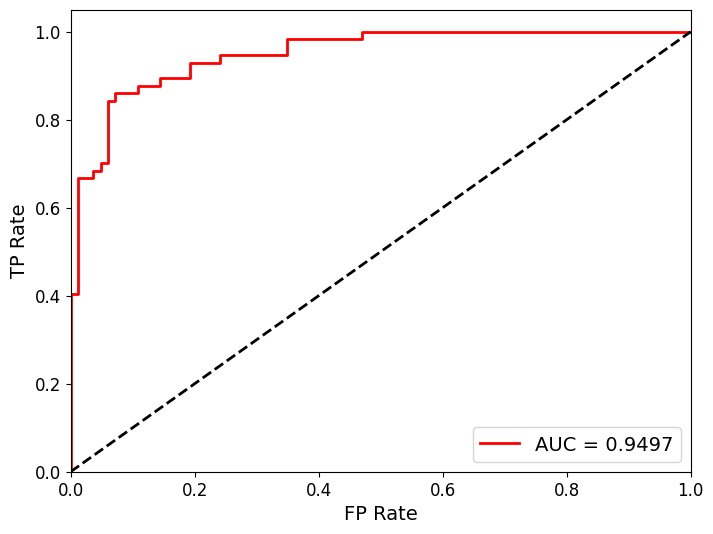
\includegraphics[width=\linewidth]{fig/BTA_roc-auc.png}
        \caption*{BTA ROC curve}
    \end{minipage}
    \hfill
    \begin{minipage}[t]{0.48\textwidth}
        \centering
        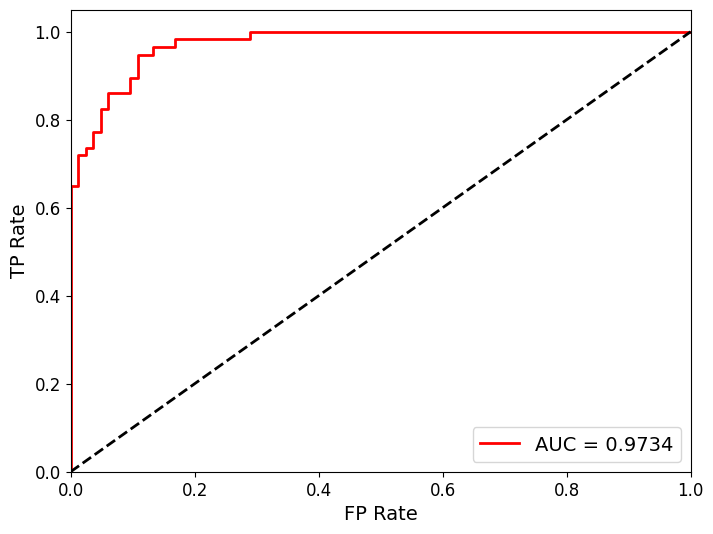
\includegraphics[width=\linewidth]{fig/BTA-combined_roc-auc.png}
        \caption*{BTA-combined ROC curve}
    \end{minipage}
    \hfill
    \begin{minipage}[t]{0.5\textwidth}
        \centering
        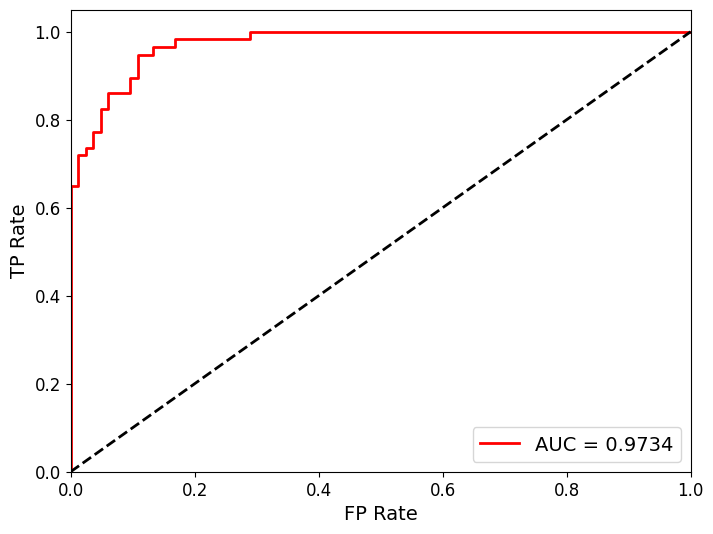
\includegraphics[width=\linewidth]{fig/BTA-combined_roc-auc.png}
        \caption*{Barlow Twins ROC curve}
    \end{minipage}
    
    \caption{Comparison of AUC ROC scores for every method}
    \label{fig:experiment}
\end{figure}

In this experiment, we set $\lambda_{BT} = 4 \cdot 10^{-3}$ for projector training loss 
function and $\lambda = 2 \cdot 10^{-5}$ for BTA-combined training. The chosen $\lambda_{BT}$ 
value is similar to the value proposed in the \cite{zbontar2021barlow} article, while 
impact of $\lambda$ value we will explore in the following section.

\section{Hyperparameter values}\label{sec:hyperval}

In this section, we conduct experiments to estimate the best hyperparameter values 
over accuracy metrics (accuracy and F1-score). While we set 
$\lambda_{BT} = 4 \cdot 10^{-3}$, which is nearly the same as in the main article's 
$\lambda_{BT}$ value (\cite{zbontar2021barlow}), we want to estimate $\lambda$ for 
BTA-combined training.

\begin{wrapfigure}{r}{0.65\textwidth}
    \centering
    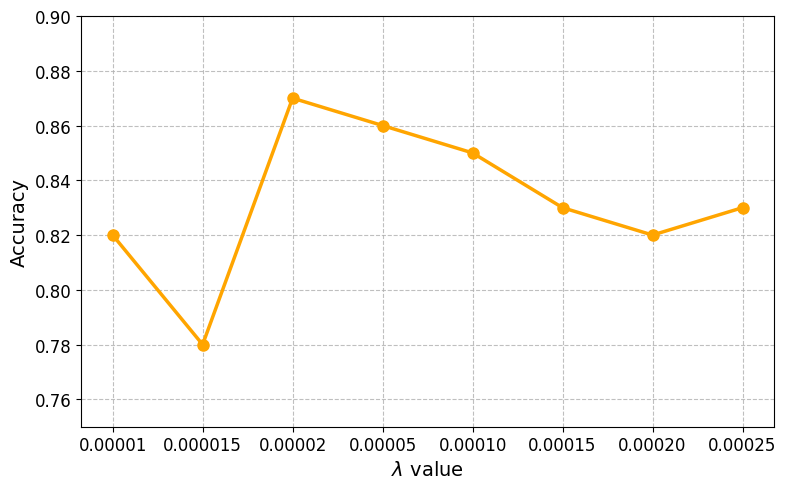
\includegraphics[width=1\linewidth]{fig/BTA-combined_lambdas-accuracy.png}
    \caption{Model accuracy varying $\lambda$ value}
\end{wrapfigure}
To determine the best value for $\lambda$, we tested multiple values during training of the BTA-combined model, running each experiment for 100 epochs. If $\lambda$ is set "too low", the projector loss barely affects training. Without this component, the model fails to learn useful features from the projector, leading to worse accuracy. However, if $\lambda$ is "too high", the BCE loss (responsible for training the classifier) gets overshadowed. This imbalance prevents the classifier from learning to make reliable predictions, even if the projector works well. After testing different values, we found that $\lambda = 2 \cdot 10^{-5}$ strikes the right balance: it allows both the projector and classifier to contribute effectively during training. At this value, the model achieves its highest accuracy compared to other tested options, as shown in Figure 2.

\begin{wrapfigure}{r}{0.65\textwidth}
    \centering
    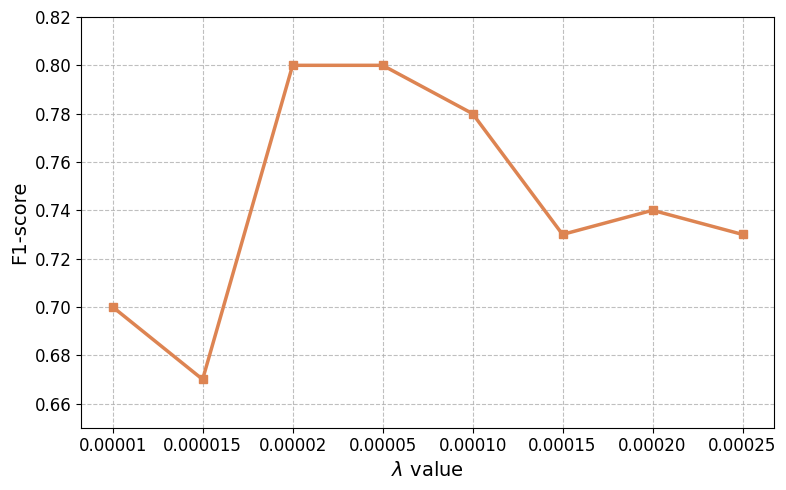
\includegraphics[width=1\linewidth]{fig/BTA-combined_lambdas-f1-score.png}
    \caption{Model F1-score varying $\lambda$ value}
\end{wrapfigure}
The F1-score curve (Figure 3) further validates the optimal choice of $\lambda = 2 \cdot 10^{-5}$, mirroring the accuracy trends. Unlike accuracy, which measures overall correctness, the F1-score balances precision and recall, making it particularly sensitive to binary classification imbalance since we set the probability of the pair of images being the same in accuracy validation to $0.4$. As was mentioned before, the sharp decline in F1-score at higher $\lambda$ values ($>10^{-4}$) suggests that an overemphasis on the projector loss destabilizes the classifier’s ability to reconcile false positives and negatives. Conversely, at lower $\lambda$ ($<2 \cdot 10^{-5}$), the F1-score somehow drops as the accuracy does indicating that residual projector regularization—even when minimal—still aids in extracting features that harmonize precision and recall. The symmetry between the accuracy and F1-score maxima underscores that $\lambda = 2 \cdot 10^{-5}$ maximizes overall performance on linear classification metrics.

\section{Conclusion}\label{sec:concl}

Our results show that our model significantly outperforms the state-of-the-art \texttt{Barlow Twins} framework \cite{zbontar2021barlow} on pairwise image comparison. The main innovation is our new training method, which uses a combined loss to jointly train a parallel projector and linear classifier. This approach performs as well as the traditional two-stage training setup. We believe future work in pairwise image comparison, especially in complex visual tasks, can benefit from our unified strategy, potentially setting a new standard for handling visually ambiguous image pairs.

%%%%%%%%%%%%%%%%%%%%%%%%%%%%%%%%%%%%%%%%%%%%%%%%%%%%%%%%%%%%

\nocite{*}

\bibliographystyle{unsrtnat}
\bibliography{references}

%%%%%%%%%%%%%%%%%%%%%%%%%%%%%%%%%%%%%%%%%%%%%%%%%%%%%%%%%%%%

%\newpage
%\appendix
%\section{Appendix / supplemental material}\label{app}
%\subsection{Additional experiments}\label{app:exp}
%TODO

\end{document}
